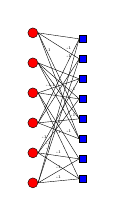
\begin{tikzpicture}
\def\horzgap{0.25in}; %Horizontal gap between nodes/levels
\def \gapVN{0.15in}; %vertical gap between nodes
\def \gapCN{0.1in}; %Horizontal gap between nodes

\def \textoffs{0.12in}; %Offset for writing text above a node
\def\nodewidth{0.05in};
\def\nodewidthA{0.05in};
\def \edgewidth{0.035in};
\def\ext{0.2in};

\def \n {8};
\def\ldeg{3};
\def\rdeg{6};
\def\langle{40};%120 degrees/3
\def\langle{20};%120 degrees/6

\tikzstyle{check} = [rectangle, draw,line width=0.05mm,  inner sep=0mm, fill=black, minimum height=\nodewidthA, minimum width=\nodewidthA]
\tikzstyle{checksm} = [rectangle, draw, line width=0.05mm, inner sep=0mm, fill=blue,minimum height=\edgewidth,minimum width=\edgewidth]

\tikzstyle{bit} = [circle, draw,line width=0.05mm, inner sep=0mm, fill=red, minimum size=\nodewidthA]
\tikzstyle{bitsm} = [circle, draw, very thin, inner sep=0mm,fill=red, minimum size=\edgewidth]
\tikzstyle{edgesock} = [circle, inner sep=0mm, minimum size=\edgewidth,draw, fill=white]     

                          
\foreach \vn in {1,...,6}{
 \node[bit] (vn\vn) at (0,\vn*\gapVN) {};
}

\foreach \cn in {1,...,8}{
\node[checksm] (cn\cn) at (\horzgap,0.07in+\cn*\gapCN) {};
}

\draw[line width=0.05mm] (vn6.east)--(cn8.west);
\draw[line width=0.05mm] (vn3.east)--(cn8.west) node[pos=0.75,above,scale=0.3]{\tiny{-1}} ;
\draw[line width=0.05mm] (vn1.east)--(cn8.west) node[pos=0.25,above,scale=0.3]{\tiny{-1}} ;

\draw[line width=0.05mm] (vn6.east)--(cn7.west) node[pos=0.75,above,scale=0.3]{\tiny{-1}} ;
\draw[line width=0.05mm] (vn3.east)--(cn7.west);
\draw[line width=0.05mm] (vn1.east)--(cn7.west) node[pos=0.25,above,scale=0.3]{\tiny{-1}} ;

\draw[line width=0.05mm] (vn5.east)--(cn6.west);
\draw[line width=0.05mm] (vn4.east)--(cn6.west) node[pos=0.25,above,scale=0.3]{\tiny{-1}} ;
\draw[line width=0.05mm] (vn2.east)--(cn6.west) node[pos=0.15,above,scale=0.3]{\tiny{-1}} ;

\draw[line width=0.05mm] (vn5.east)--(cn5.west) node[pos=0.85,above,scale=0.3]{\tiny{-1}} ;
\draw[line width=0.05mm] (vn4.east)--(cn5.west);
\draw[line width=0.05mm] (vn2.east)--(cn5.west) node[pos=0.5,above,scale=0.3]{\tiny{-1}} ;

\draw[line width=0.05mm] (vn6.east)--(cn4.west) node[pos=0.25,above,scale=0.3]{\tiny{-1}} ;
\draw[line width=0.05mm] (vn5.east)--(cn4.west);
\draw[line width=0.05mm] (vn3.east)--(cn4.west) node[pos=0.85,above,scale=0.3]{\tiny{-1}} ;

\draw[line width=0.05mm] (vn6.east)--(cn3.west);
\draw[line width=0.05mm] (vn5.east)--(cn3.west) node[pos=0.35,above,scale=0.3]{\tiny{-1}} ;
\draw[line width=0.05mm] (vn3.east)--(cn3.west) node[pos=0.75,above,scale=0.3]{\tiny{-1}} ;


\draw[line width=0.05mm] (vn4.east)--(cn2.west);
\draw[line width=0.05mm] (vn2.east)--(cn2.west)node[pos=0.5,above,scale=0.3]{\tiny{-1}} ;
\draw[line width=0.05mm] (vn1.east)--(cn2.west)node[pos=0.5,above,scale=0.3]{\tiny{-1}} ;

\draw[line width=0.05mm] (vn1.east)--(cn1.west)node[pos=0.5,above,scale=0.3]{\tiny{-1}} ;
\draw[line width=0.05mm] (vn2.east)--(cn1.west);
\draw[line width=0.05mm] (vn4.east)--(cn1.west)node[pos=0.5,above,scale=0.3]{\tiny{-1}} ;

\end{tikzpicture}